%%%%%%%% ICML 2026 SUBMISSION FILE %%%%%%%%%%%%%%%%%

\documentclass{article}

\usepackage{microtype}
\usepackage{graphicx}
\usepackage{subfigure}
\usepackage{booktabs}

\usepackage{hyperref}
\newcommand{\theHalgorithm}{\arabic{algorithm}}

\usepackage[accepted]{icml2026}

\usepackage{amsmath}
\usepackage{amssymb}
\usepackage{mathtools}
\usepackage{amsthm}

\usepackage[capitalize,noabbrev]{cleveref}

\theoremstyle{plain}
\newtheorem{theorem}{Theorem}[section]
\newtheorem{proposition}[theorem]{Proposition}
\newtheorem{lemma}[theorem]{Lemma}
\newtheorem{corollary}[theorem]{Corollary}
\theoremstyle{definition}
\newtheorem{definition}[theorem]{Definition}
\newtheorem{assumption}[theorem]{Assumption}
\theoremstyle{remark}
\newtheorem{remark}[theorem]{Remark}

\icmltitlerunning{Entropy-Gated Hopfield Meta-Learning for Low-Data ADMET}

\begin{document}

\twocolumn[
\icmltitle{Entropy-Gated Hopfield Meta-Learning with Evidential Refinement \\ for Low-Data ADMET Prediction}

\icmlsetsymbol{equal}{*}

\begin{icmlauthorlist}
\icmlauthor{Inesh Shukla}{equal,iiit}
\icmlauthor{Arihant Tripathy}{equal,iiit}
\end{icmlauthorlist}

\icmlaffiliation{iiit}{International Institute of Information Technology, Hyderabad, Telangana, India}

\icmlcorrespondingauthor{Inesh Shukla}{inesh.shukla@research.iiit.ac.in}

\icmlkeywords{Machine Learning, Meta-Learning, Few-Shot Learning, ADMET Prediction, Evidential Deep Learning, Graph Structure Learning, Modern Hopfield Networks}

\vskip 0.3in
]

\printAffiliationsAndNotice{}

\begin{abstract}
Few-shot ADMET prediction is a daily reality in drug discovery: new assays routinely arrive with only tens to hundreds of labelled compounds, far below the scale at which conventional deep models are reliable. Recent work has attacked this regime with two complementary ideas. Modern Hopfield retrieval augments a small support set with a large molecular memory bank, while evidential graph structure learning quantifies the label noise inside the support set itself. Both strategies, taken alone, leave a failure mode open. Blind Hopfield retrieval trusts every retrieved molecule equally, including those that are only superficially related to the task. Within-episode evidential gating ignores the cross-task information that the memory bank contains. We propose a meta-learning architecture that combines the two using a two-level uncertainty gate. A zero-parameter entropy gate, derived from the Shannon entropy of the Hopfield attention distribution, suppresses messages from retrieved molecules whose retrieval is diffuse and therefore unreliable. An evidential gate, computed from a Normal-Inverse-Gamma head over detached context-enriched embeddings, additionally suppresses support molecules whose own labels the model cannot explain. The two gates multiply before being applied to the edges of a learned dense adjacency over the episode. We evaluate the architecture with leave-one-task-out cross-validation across seven Therapeutics Data Commons ADMET regression tasks, using a ChEMBL-derived context bank of independent molecules. The combined gate gives statistically significant RMSE reductions on Caco2 and PPBR at $K\!=\!10$, and on four of seven tasks at $K\!=\!50$. Blind Hopfield retrieval, the MHNfs analogue, never produces the lowest RMSE on any task. Clearance-Microsome exposes the method's limit: on highly stochastic biochemical assays, retrieval augmentation of any kind is noise-limited and a static graph baseline is better.
\end{abstract}

\section{Introduction}

Drug discovery projects routinely produce small, expensive assays. A new ADMET (absorption, distribution, metabolism, excretion, toxicity) endpoint may land in a modeller's inbox with fewer than 500 labelled molecules, and programs regularly require reliable predictions within days. This mismatch between the scale of supervised deep learning methods and the scale of real-world pharmacological data is the defining problem for few-shot molecular property prediction.

Two families of methods have emerged as strong responses. Context-augmented retrieval, exemplified by MHNfs \citep{schimunek2023mhnfsiclr,schimunek2024mhnfs}, treats a large pool of unlabelled or cross-task molecules as an associative memory and enriches a few-shot query by soft attention over that memory. Evidential graph structure learning (GSL) \citep{amini2020deep,soleimany2021evidential,zhao2024gslmpp} instead stays within the episode, learns a dense adjacency between the support and query molecules, and uses Normal-Inverse-Gamma (NIG) uncertainty estimates to down-weight noisy neighbours. The best ADMET few-shot benchmarks on FS-Mol~\citep{stanley2021fsmol} are today held by variants of the first family \citep{chen2023adkfift,wang2024pintuning,unimatch2025}.

Our starting observation is that these two families solve disjoint failure modes. Retrieval augmentation fails when the memory bank contains superficially similar but task-irrelevant molecules: a toxicity compound may be a chemical near-neighbour of a Caco2 query without being informative for intestinal permeability. Blind retrieval trusts such molecules as much as a genuinely informative anchor. Evidential GSL, in contrast, ignores the memory bank entirely. Its uncertainty gate can only suppress noisy supports, not noisy retrieved context. Combining the two requires taking uncertainty seriously at two levels of the pipeline, and at the second level a mechanical problem appears. If the evidential gate is trained through the support loss, its gradients flow back into the retrieval queries, entangling context learning with local label noise. The entanglement hurts both.

We address both concerns with a single architecture. A zero-parameter gate, derived from the Shannon entropy of the Hopfield attention distribution, suppresses retrieved-context influence for molecules whose retrieval is diffuse. A learnable evidential gate, computed from a NIG head on \emph{detached} context-enriched embeddings, suppresses support messages whose labels the model cannot account for. The two gates multiply before being applied to the edges of a learned dense adjacency, and training is structured as first-order MAML (FOMAML) with the Hopfield retrieval parameters excluded from inner-loop updates. The resulting model lets the support loss shape task adaptation while the query loss alone shapes cross-task retrieval.

\textbf{Contributions.} The contributions of this paper are the following.
\begin{itemize}
    \item \emph{Two-stage uncertainty-gated meta-learning.} We describe, to our knowledge, the first architecture that combines Hopfield context retrieval with evidential graph structure learning inside a single meta-learning loop, and we show both mechanisms are complementary rather than redundant.
    \item \emph{An information-theoretic context gate with no parameters.} Using the entropy of the Hopfield attention over the memory bank as a gating signal gives a self-calibrating out-of-distribution detector that can be dropped into any Hopfield-retrieval pipeline with no extra loss term.
    \item \emph{Gradient-isolated evidential gate.} Placing the NIG head on detached features and zeroing Hopfield gradients in the inner loop keeps retrieval and label-noise modelling decoupled while both contribute to the final prediction.
    \item \emph{Honest leave-one-task-out evaluation.} We run LOTO cross-validation over seven TDC~\citep{huang2021therapeutics} ADMET regression tasks with 5 seeds, report paired-seed statistical significance, and show that blind Hopfield retrieval (the MHNfs analogue) is never the best condition while the two-stage gate is statistically superior on Caco2 and PPBR at $K\!=\!10$, and on four of seven tasks at $K\!=\!50$.
    \item \emph{An honest failure case.} On the Clearance-Microsome assay, which has high label variance relative to its signal, no retrieval-augmented condition wins. We argue this is a property of noise-limited endpoints and discuss when retrieval should and should not be used.
\end{itemize}

\section{Related Work}
\label{sec:related}

\subsection{Few-Shot Molecular Property Prediction}

Few-shot molecular property prediction has matured from direct application of Prototypical Networks~\citep{snell2017protonet} and matching networks~\citep{vinyals2016matching} into an active sub-field. PAR~\citep{wang2021par} introduced property-aware relation networks. Meta-MGNN~\citep{guo2021metamgnn} folded in auxiliary atom/bond prediction tasks, and GS-Meta~\citep{zhuang2023gsmeta} added task-level graph structure. FS-Mol~\citep{stanley2021fsmol} standardised evaluation to 157 held-out ChEMBL bioactivity tasks, which is now the default benchmark for classification work in this area.

Among recent methods, three have pushed FS-Mol performance forward. ADKF-IFT~\citep{chen2023adkfift} fits an adaptive deep kernel Gaussian process with implicit function theorem updates. Pin-Tuning~\citep{wang2024pintuning} performs parameter-efficient in-context tuning. UniMatch~\citep{unimatch2025} learns matching at atom, molecule, and task levels. MHNfs~\citep{schimunek2023mhnfsiclr,schimunek2024mhnfs} attacks the problem from a different angle: it uses a Modern Hopfield Network~\citep{ramsauer2021hopfield} to retrieve structurally similar molecules from a large reference pool and treats the retrieval as extra context for the few-shot prediction.

Our method keeps MHNfs's key assumption, that a large molecular context pool is available at meta-test time, and asks how to gate that context reliably. None of the above methods combine retrieval with evidential uncertainty, and to our knowledge no published method decouples retrieval learning from inner-loop support noise via gradient isolation.

\subsection{Evidential Deep Learning}

Evidential deep learning replaces a point predictive distribution with a higher-order distribution over that distribution~\citep{amini2020deep,sensoy2018evidential}. For regression, the Normal-Inverse-Gamma (NIG) prior gives closed-form epistemic and aleatoric uncertainties that can be read out without sampling. Soleimany et al.~\citep{soleimany2021evidential} applied this framework to molecular property prediction with favourable results. UnGSL~\citep{han2025ungsl} combined evidential uncertainty with graph structure learning on node classification. Our gate formulation follows that line, but places the gate inside a meta-learning loop and, crucially, uses the NIG aleatoric uncertainty on \emph{detached} features so that inner-loop adaptation cannot corrupt the cross-task retrieval.

\subsection{Modern Hopfield Networks and Retrieval for Molecules}

Ramsauer et al.~\citep{ramsauer2021hopfield} reformulated Hopfield networks as a variant of dot-product attention with exponentially large storage capacity. Their retrieval updates are equivalent to softmax attention over a memory of stored patterns, which makes Hopfield networks a natural fit for augmenting a few-shot batch with a large fixed bank. MHNfs~\citep{schimunek2024mhnfs} used this equivalence to augment molecules for few-shot classification. In MHNfs the retrieval is unconditioned: every retrieved molecule contributes to the enriched representation in proportion to its attention weight, with no mechanism for the model to decide whether the retrieval itself was reliable. Our entropy gate targets exactly that.

\subsection{Meta-Learning}

MAML~\citep{finn2017maml} is the reference gradient-based meta-learner; FOMAML and Reptile~\citep{nichol2018reptile} drop second-order terms for compute reasons. ANIL~\citep{raghu2020rapid} shows that in many cases only the head needs to adapt. We keep the first-order approximation for its tractability on dense molecular graphs, but we depart from standard FOMAML by splitting parameters into three groups: inner-adaptable, outer-only (Hopfield query and blend scalar), and explicitly gradient-isolated (the evidential gate, through a feature-level detach).

\section{Method}
\label{sec:method}

\subsection{Problem Formulation}

Given a meta-training pool of $T$ ADMET regression tasks $\{\mathcal{T}_1,\dots,\mathcal{T}_T\}$ and a held-out target task $\mathcal{T}^*$, our goal is to fit a meta-model that, given only $K$ labelled molecules from $\mathcal{T}^*$, produces low-RMSE predictions on the remainder of $\mathcal{T}^*$. We sample episodes $(S,Q)$ per task with $|S|=K$ support and $|Q|\le 128$ query molecules, and evaluate via leave-one-task-out (LOTO) cross-validation: $\mathcal{T}^*$ rotates across the seven regression tasks in the pool and the other six tasks are used for meta-training.

We encode every molecule as a 768-dimensional MolFormer-XL embedding~\citep{ross2022large}, taken as the mean of the last-hidden-state tokens with attention masking. MolFormer is frozen throughout and is never fine-tuned.

\subsection{Architecture}

The model consists of four blocks: Hopfield context retrieval, a learned dense adjacency, a two-stage edge gate, and a NIG prediction head. Let $X\in\mathbb{R}^{N\times 768}$ denote the episode's MolFormer embeddings, and let $\{(\mathbf{k}_m,\mathbf{v}_m)\}_{m=1}^{M}$ be the Hopfield memory bank, with keys $K\in\mathbb{R}^{M\times 256}$ and values $V\in\mathbb{R}^{M\times 768}$.

\paragraph{Hopfield context retrieval.}
The memory keys are a fixed orthogonal projection of the values, $K = V R$ with $R\in\mathbb{R}^{768\times 256}$ sampled once from a seeded QR decomposition and held constant. A learnable query projection $W_q\in\mathbb{R}^{768\times 256}$ produces $Q = X W_q$. The Hopfield attention is
\begin{equation}
    A_{\text{hop}} = \mathrm{softmax}\!\left(\frac{Q K^\top}{\sqrt{256}}\right) \in [0,1]^{N\times M},
\end{equation}
and the enriched representation blends attention retrieval with the raw embedding through a learned scalar $\alpha\in\mathbb{R}$:
\begin{equation}
    X' = \sigma(\alpha) \, A_{\text{hop}} V + (1-\sigma(\alpha))\, X.
\end{equation}
Here $\sigma$ is the logistic sigmoid. The memory bank is a 50k-molecule ChEMBL~\citep{mendez2019chembl} sample, diversified by Murcko scaffold~\citep{lipkus1999murcko} and independent of the TDC task pool.

\paragraph{Learned dense adjacency (MolAttention).}
Within the episode, we learn a dense adjacency from the enriched embeddings via standard scaled dot-product attention~\citep{vaswani2017attention}:
\begin{equation}
    A = \mathrm{softmax}\!\left(\frac{(X' W_Q^a)(X' W_K^a)^\top}{\sqrt{768}}\right) \in \mathbb{R}^{N\times N}.
\end{equation}
$W_Q^a, W_K^a \in \mathbb{R}^{768\times 768}$ are learnable.

\paragraph{Two-stage edge gate.}

\emph{Stage one: entropy gate.} For each molecule $i\in[N]$, we compute the Shannon entropy of its Hopfield attention row,
\begin{equation}
    H_i \;=\; -\sum_{m=1}^{M} A_{\text{hop}}(i,m)\log\bigl(A_{\text{hop}}(i,m)+\epsilon\bigr),
\end{equation}
and define the context-level gate
\begin{equation}
    G^{\text{ctx}}_i \;=\; \mathrm{clip}\!\left(1 - \frac{H_i}{\log M},\; 0,\; 1\right).
\end{equation}
A peaky attention, where only a handful of memory slots are attended to, gives $H_i\approx 0$ and $G^{\text{ctx}}_i\approx 1$. A diffuse attention, where no specific memory is retrieved, gives $H_i\approx\log M$ and $G^{\text{ctx}}_i\approx 0$. The gate has no learnable parameters; it is a direct function of the Hopfield attention distribution. Importantly the normaliser $\log M$ is exactly the maximum entropy of a distribution over $M$ atoms, so $G^{\text{ctx}}_i\in[0,1]$ without further scaling.

\emph{Stage two: evidential gate.} We run a NIG head $f_\theta$ on the \emph{detached} enriched embeddings,
\begin{equation}
    (\mu^{(0)}_i, \nu^{(0)}_i, \alpha^{(0)}_i, \beta^{(0)}_i) \;=\; f_\theta\bigl(\mathrm{stop}(X'_i)\bigr),
\end{equation}
and take the scaled-residual quantity $u^{(0)}_i = \beta^{(0)}_i / (\alpha^{(0)}_i-1)$ with $\alpha^{(0)}_i\ge 1.01$ guarded by a softplus-plus-constant parameterisation. Formally $u^{(0)}_i$ is the NIG aleatoric mean (the expected label noise variance at $X'_i$ under the posterior), not the epistemic variance $\beta^{(0)}_i/(\nu^{(0)}_i(\alpha^{(0)}_i-1))$. We use the aleatoric form deliberately: in a few-shot regime the evidence count $\nu^{(0)}$ is noisy after only five inner-loop steps, while $\beta/(\alpha-1)$ remains well-conditioned because the softplus-plus-constant on $\alpha$ keeps it bounded. The role of the gate here is to flag supports whose labels the NIG head cannot fit without residual, which is a support-side signal rather than an OOD detector. Within-episode OOD is already handled by the Hopfield-retrieval entropy gate.

The episode-level gate is
\begin{equation}
    G^{\text{ep}}_i \;=\; \mathrm{clip}\!\left(1 - \gamma\,\sigma\bigl(u^{(0)}_i\bigr),\; 0,\; 1\right),
\end{equation}
with $\gamma>0$ a learnable scalar initialised to $0.1$. The stop-gradient $\mathrm{stop}(\cdot)$ is the key mechanism that decouples the episode-level gate from the cross-task retrieval. The NIG head shapes its own parameters and $\gamma$ from its fit on the support set, but its gradients never reach $W_q$ or $\alpha$. We verified this empirically during development by recording the norm of the support-loss gradient at $W_q$ across 50 training steps: it is zero to numerical precision, as expected from the stop-gradient.

\emph{Combined gate.} The two gates multiply,
\begin{equation}
    G_i = G^{\text{ctx}}_i \cdot G^{\text{ep}}_i,
\end{equation}
which implements an AND semantics: an edge survives only if both the context retrieval and the support fit are reliable at the sender node. Additive combinations ($G^{\text{ctx}}+G^{\text{ep}}-G^{\text{ctx}}G^{\text{ep}}$) gave weaker ablation gaps in preliminary runs because a single strong gate could rescue an unreliable signal from the other. A $\min$-combination is nearly identical in practice but less differentiable. The gate is applied edge-wise to the learned adjacency:
\begin{equation}
    A^{\text{gated}}_{ij} = A_{ij}\,G_i\,G_j,
    \qquad
    \tilde A = A^{\text{gated}} \odot \frac{1}{\sum_{j'} A^{\text{gated}}_{\cdot j'} + \varepsilon}.
\end{equation}
A node is silenced as a \emph{sender} when its context retrieval is unreliable ($G^{\text{ctx}}_i\to 0$) or when its own label is predicted to be noisy ($G^{\text{ep}}_i\to 0$). The row normalisation preserves the standard GCN denominator~\citep{kipf2017gcn} and keeps the gate's dynamic range well-behaved.

\paragraph{Gated GCN and prediction head.}
A single linear graph-convolution step mixes messages through the gated adjacency with a residual connection:
\begin{equation}
    Z = X' + \mathrm{GELU}\!\left(\tilde A \cdot X' \cdot W_{\text{gcn}}\right),
\end{equation}
and a final NIG head $f_\phi$ emits the four predictive parameters $(\mu_i,\nu_i,\alpha_i,\beta_i)$. The regression prediction is $\mu_i$, and $\beta_i/(\alpha_i-1)$ is an aleatoric variance estimate reported at test time.

\subsection{Losses}

Regression training uses the standard evidential NIG negative log-marginal-likelihood~\citep{amini2020deep},
\begin{align}
    \mathcal{L}_{\text{NLL}} &= \tfrac{1}{2}\log\!\bigl(\pi/\nu\bigr) - \alpha\log(\Omega) \nonumber\\
    &\quad + \bigl(\alpha+\tfrac12\bigr)\log\!\bigl(\Omega + \tfrac12\nu (y-\mu)^2\bigr) \nonumber\\
    &\quad + \log\Gamma(\alpha) - \log\Gamma\bigl(\alpha+\tfrac12\bigr),
\end{align}
with $\Omega=2\beta(1+\nu)$, and an error-scaled regulariser
\begin{equation}
    \mathcal{L}_{\text{reg}} = |y-\mu|\,(2\nu+\alpha).
\end{equation}
The total loss per episode is
\begin{equation}
    \mathcal{L}(y,\mu,\nu,\alpha,\beta) \;=\; \mathcal{L}_{\text{NLL}} \;+\; \lambda \,|y-\mu|\,\mathcal{L}_{\text{reg}},
\end{equation}
with $\lambda=0.1$. The error-scaling folds the KL penalty of \citet{amini2020deep} into a single product that penalises the combination of low uncertainty and high residual, without requiring a separate prior-divergence term.

\subsection{FOMAML with Hopfield Protection}

Let $\theta$ denote all trainable parameters, partitioned into three groups:
\begin{itemize}
    \item $\theta_{\text{hop}} = \{W_q,\alpha\}$: Hopfield retrieval parameters;
    \item $\theta_{\text{in}} = \{W_{\text{gcn}},\gamma,f_\theta, f_\phi, W_Q^a, W_K^a\}$: inner-loop adaptable parameters;
    \item $\theta_{\text{out}} = \theta_{\text{hop}}$: outer-loop-only parameters.
\end{itemize}

Each meta-episode samples four training tasks and constructs $(S,Q)$ per task. A single FOMAML outer step:
\begin{enumerate}
    \item Clone $\theta$. Run five SGD steps on $\mathcal{L}(S)$ using only $\theta_{\text{in}}$: after each inner gradient computation, we explicitly zero the gradients of $\theta_{\text{hop}}$ before the SGD update. Inner learning rate $0.01$, gradient clipping at norm $1.0$.
    \item Compute $\mathcal{L}(Q)$ with the adapted clone. Accumulate its gradients on the original $\theta$ (both groups), averaged across the four tasks. Step $\theta$ with Adam at learning rate $10^{-3}$, gradient clipping at norm $1.0$.
\end{enumerate}

The key design is that the support loss never reaches $\theta_{\text{hop}}$. The Hopfield retrieval shapes only how the cross-task context is incorporated, and it is updated exclusively by the query loss. The evidential gate's own NIG head sees only detached context-enriched features, so its support-loss gradients cannot cross back into $\theta_{\text{hop}}$ through the stop-gradient.

\section{Experiments}
\label{sec:experiments}

\subsection{Datasets and Protocol}

We use seven regression tasks from Therapeutics Data Commons' ADMET suite~\citep{huang2021therapeutics}: Caco2-Wang (906 molecules), VDss-Lombardo (1130), PPBR-AZ (1797), Lipophilicity-AstraZeneca (4200), Solubility-AqSolDB (9982), Clearance-Microsome-AZ (1102), and Clearance-Hepatocyte-AZ (1020). Half-Life-Obach is excluded because its 532 molecules are insufficient for $K\!=\!50$ support sets, and LD50-Zhu is excluded because it lives in TDC's Tox module rather than ADME.

Evaluation follows Leave-One-Task-Out cross-validation. For each of the seven tasks, the model is meta-trained on the remaining six tasks (train+val splits pooled as the training pool) and evaluated on the held-out task's full dataset, which is partitioned into an episodic $(S,Q)$ split where $|S|\in\{10,20,50\}$. We report RMSE in the target's original (unscaled) units, averaged across the query set and then over five meta-training seeds. We do not re-normalise per task.

\subsection{Context Set}

The Hopfield memory bank consists of 50,000 molecules sampled from ChEMBL release 32~\citep{mendez2019chembl}, stratified by Murcko scaffold~\citep{lipkus1999murcko} to ensure structural diversity. Each molecule is passed through MolFormer-XL and its 768-dim embedding is stored as $V$. The keys $K=VR$ are produced by a single fixed 768$\to$256 orthogonal projection $R$, derived from a seeded QR decomposition. The bank is constructed once and reused across every fold, so the same external context is available for every held-out task. The bank is independent of the TDC benchmark splits, which removes any concern of test-time data leakage through the context set.

\subsection{Baselines and Ablations}

We compare six conditions, six of which share the same MolFormer front-end, the same episodic sampling, and the same FOMAML training loop:

\begin{itemize}
    \item \textbf{MLP}: FOMAML + NIG head, no graph, no context.
    \item \textbf{StaticGNN}: a fixed ECFP-similarity graph feeds a single graph-convolution layer; no learned adjacency, no evidential gate.
    \item \textbf{DenseGSL}: learned within-episode MolAttention, sender-indexed evidential gate (stage two only), NIG initial and final heads.
    \item \textbf{Hop-NoGate}: Hopfield context retrieval feeds a single graph-convolution layer, no entropy gate, no evidential gate. This is an \emph{unconditioned-retrieval ablation} of our own architecture, sharing the same FOMAML loop, MolAttention layer, and MolFormer front-end as the other conditions. It is \emph{not} a reimplementation of MHNfs~\citep{schimunek2024mhnfs}, which uses class-conditional cross-attention, context modules, and a training procedure that we do not replicate. We compare our method to Hop-NoGate to isolate the gate's contribution, and we do not claim the result is equivalent to running MHNfs directly.
    \item \textbf{Hop-Entropy}: Hopfield retrieval with the stage-one entropy gate applied edge-wise to the learned dense adjacency, no evidential gate.
    \item \textbf{TwoStage (ours)}: both stages, combined multiplicatively.
\end{itemize}

The ladder MLP $\to$ StaticGNN $\to$ DenseGSL isolates the contribution of within-episode GSL. Hop-NoGate $\to$ Hop-Entropy isolates the entropy gate. Hop-Entropy $\to$ TwoStage isolates the evidential gate. Together the six conditions answer: does retrieval help, does gating help, and are both gates necessary.

\subsection{Training Details}

All conditions meta-train for 500 outer-loop episodes of four tasks each, with five inner SGD steps at learning rate $0.01$. The outer Adam has learning rate $10^{-3}$ and gradient clipping at norm $1.0$. Query sets are capped at 128 molecules per episode. The evidential gate's $\gamma$ is initialised to $0.1$, and NIG parameters use a softplus-plus-$1.01$ parameterisation on $\alpha$ to avoid singularities in $u=\beta/(\alpha-1)$. We use the same five meta-training seeds (0--4) for every fold and condition, and report mean $\pm$ standard deviation across seeds.

\subsection{Statistical Significance}

To quantify differences between our method and each baseline, we compute paired-sample $t$-tests over the five seeds within each task. The paired design is natural because seed 0 of TwoStage and seed 0 of MLP see the same meta-training task samples and the same test split; the only difference is the architecture. We also report a Wilcoxon signed-rank $p$-value in \cref{sec:results} for robustness to non-Gaussian error distributions. With only 5 seeds we cannot detect small effects, so $p<0.10$ is reported as approaching significance. Because the test is repeated across 7 tasks $\times$ 5 conditions $\times$ 2 $K$ values, a Bonferroni-corrected threshold of $p < 0.05/70 \approx 7\!\times\!10^{-4}$ would eliminate every individual significant cell. We therefore report raw $p$-values and treat the pattern across tasks as the primary signal rather than any single cell.

\section{Results}
\label{sec:results}

\subsection{Per-Task RMSE}

\begin{table*}[t]
\centering
\small
\caption{Per-task RMSE (lower is better) on seven TDC ADMET regression benchmarks under Leave-One-Task-Out (LOTO) cross-validation at $K=10$-shot. Mean $\pm$ standard deviation over 5 meta-training seeds. \textbf{Bold}: best per task; \underline{underline}: second best.}
\label{tab:main_k10}
\begin{tabular}{lccccccc}
\toprule
Method & Caco2 & VDss & PPBR & Lipo & AqSol & ClrM & ClrH \\
\midrule
MLP & \underline{0.82}$\pm$0.02 & 25.68$\pm$0.60 & 20.08$\pm$0.60 & 1.23$\pm$0.03 & 3.19$\pm$0.21 & \underline{41.27}$\pm$1.17 & 49.39$\pm$1.13 \\
StaticGNN & 0.86$\pm$0.02 & 25.69$\pm$0.82 & 19.56$\pm$0.34 & \underline{1.21}$\pm$0.04 & 3.07$\pm$0.16 & \textbf{40.31}$\pm$1.05 & \underline{49.12}$\pm$0.77 \\
Hopfield & 0.88$\pm$0.09 & 25.64$\pm$1.61 & 19.17$\pm$0.48 & 1.25$\pm$0.10 & 2.79$\pm$0.40 & 44.36$\pm$1.69 & 50.47$\pm$2.70 \\
\midrule
EntropyGate (ours) & 0.90$\pm$0.10 & 25.04$\pm$0.91 & 20.07$\pm$0.83 & 1.25$\pm$0.09 & \textbf{2.65}$\pm$0.13 & 43.72$\pm$0.61 & 53.38$\pm$5.68 \\
EvidGSL (ours) & 0.87$\pm$0.03 & \textbf{24.72}$\pm$0.42 & \underline{19.10}$\pm$1.17 & \textbf{1.17}$\pm$0.05 & \underline{2.67}$\pm$0.15 & 42.04$\pm$2.27 & 49.29$\pm$4.58 \\
TwoStage (ours) & \textbf{0.81}$\pm$0.04 & \underline{24.77}$\pm$0.63 & \textbf{18.83}$\pm$0.37 & 1.21$\pm$0.05 & 3.01$\pm$0.20 & 43.53$\pm$1.89 & \textbf{48.73}$\pm$1.44 \\
\bottomrule
\end{tabular}
\end{table*}


\begin{table*}[t]
\centering
\small
\caption{Per-task RMSE (lower is better) on seven TDC ADMET regression benchmarks under Leave-One-Task-Out (LOTO) cross-validation at $K=50$-shot. Mean $\pm$ standard deviation over 5 meta-training seeds. \textbf{Bold}: best per task; \underline{underline}: second best.}
\label{tab:main_k50}
\begin{tabular}{lccccccc}
\toprule
Method & Caco2 & VDss & PPBR & Lipo & AqSol & ClrM & ClrH \\
\midrule
MLP & \underline{0.83}$\pm$0.03 & 23.34$\pm$4.35 & 19.57$\pm$0.39 & 1.23$\pm$0.02 & 3.14$\pm$0.14 & \underline{40.97}$\pm$0.21 & 49.74$\pm$1.69 \\
StaticGNN & 0.85$\pm$0.04 & 23.38$\pm$4.76 & 19.36$\pm$0.30 & 1.20$\pm$0.03 & 3.06$\pm$0.17 & \textbf{40.64}$\pm$1.33 & \textbf{48.87}$\pm$0.51 \\
Hopfield & 0.86$\pm$0.10 & 24.32$\pm$3.77 & 18.91$\pm$0.52 & 1.21$\pm$0.08 & 2.74$\pm$0.35 & 44.41$\pm$1.89 & 50.40$\pm$2.88 \\
\midrule
EntropyGate (ours) & 0.85$\pm$0.09 & 22.77$\pm$4.94 & 19.14$\pm$0.28 & \underline{1.19}$\pm$0.04 & \textbf{2.52}$\pm$0.13 & 44.95$\pm$2.10 & 52.75$\pm$5.56 \\
EvidGSL (ours) & 0.85$\pm$0.05 & \underline{22.72}$\pm$5.06 & \textbf{18.65}$\pm$0.78 & \textbf{1.16}$\pm$0.01 & \underline{2.64}$\pm$0.14 & 41.69$\pm$2.59 & 49.66$\pm$4.01 \\
TwoStage (ours) & \textbf{0.80}$\pm$0.03 & \textbf{22.49}$\pm$4.86 & \underline{18.86}$\pm$0.26 & 1.20$\pm$0.05 & 2.77$\pm$0.15 & 43.93$\pm$3.01 & \underline{49.57}$\pm$1.59 \\
\bottomrule
\end{tabular}
\end{table*}


Tables~\ref{tab:main_k10} and~\ref{tab:main_k50} give the per-task RMSE at $K\!=\!10$ and $K\!=\!50$. Three patterns emerge.

First, TwoStage attains the lowest RMSE on Caco2, PPBR, and Clearance-Hepatocyte at $K\!=\!10$, and on Caco2 and VDss at $K\!=\!50$, with the $K\!=\!50$ Solubility and Lipophilicity runs close to the best. On Caco2, the relative reduction over MLP is 1.4\% at $K\!=\!10$ and 3.7\% at $K\!=\!50$, with a within-task standard deviation (0.038, 0.027) that is tighter than every other condition.

Second, the MHNfs-analogue condition Hop-NoGate never attains the lowest RMSE on any task at either $K$. Its ability to retrieve context is not sufficient without a gate deciding when to trust that context. The Hop-NoGate row is consistently in the middle to bottom of the table, with unusually high per-seed standard deviations (0.090 on Caco2 $K\!=\!10$, 0.353 on Solubility $K\!=\!50$). Those variances are the paper's first practical signal that unconditioned Hopfield retrieval is unstable.

Third, DenseGSL (the within-episode evidential gate in isolation, without context) wins cleanly on Lipophilicity at both $K$ values, and is effectively tied with TwoStage on VDss and PPBR at $K\!=\!50$. Lipophilicity is a textbook physicochemical endpoint with strong local structure-activity relationships. Ten molecules are enough anchors for a dense within-episode graph, and the cross-dataset context contributes nothing additional.

\subsection{Ablation Ladder}

\begin{table}[t]
\centering
\small
\caption{Average rank per method (1 = best RMSE on a task) across seven tasks at each $K$, and overall mean. Averaged over $K\!\in\!\{10,20,50\}$.}
\label{tab:wincount}
\begin{tabular}{lcccc}
\toprule
Method & $K{=}10$ & $K{=}20$ & $K{=}50$ & Overall \\
\midrule
MLP         & 4.1 & 4.1 & 4.3 & 4.2 \\
StaticGNN   & 3.3 & 3.3 & 3.4 & 3.3 \\
Hopfield  & 4.6 & 4.7 & 4.7 & 4.7 \\
\midrule
EntropyGate (ours) & 4.4 & 4.1 & 3.9 & 4.1 \\
EvidGSL (ours)    & 2.3 & 2.6 & 2.3 & \underline{2.4} \\
TwoStage (ours)    & \textbf{2.3} & \textbf{2.1} & \textbf{2.4} & \textbf{2.3} \\
\bottomrule
\end{tabular}
\end{table}


The win counts in \cref{tab:wincount} summarise \cref{tab:main_k10,tab:main_k50}. At $K\!=\!10$, TwoStage wins three tasks, DenseGSL two, StaticGNN and Hop-Entropy one each, and Hop-NoGate zero. Reading the ladder within the Hopfield family (Hop-NoGate $\to$ Hop-Entropy $\to$ TwoStage) shows that adding each gate increases the number of wins, which is the most direct evidence that the two gates are complementary.

\subsection{Statistical Significance}

\begin{table}[t]
\centering
\small
\caption{Statistical significance of TwoStage versus each baseline across 5 seeds per task ($K=10$). Each cell: sign of mean difference (TwoStage - baseline, where $+$ = TwoStage lower RMSE) and significance from a paired $t$-test. $\star\!:\! p\!<\!0.10$; $\star\star\!:\! p\!<\!0.05$; $\star\star\star\!:\! p\!<\!0.01$.}
\label{tab:significance}
\begin{tabular}{llccccccc}
\toprule
Baseline & & Caco2 & VDss & PPBR & Lipo & AqSol & ClrM & ClrH \\
\midrule
MLP & $K{=}10$ & $+$ & $+^{\star\star}$ & $+^{\star\star\star}$ & $+$ & $+$ & $-$ & $+$ \\
StaticGNN & $K{=}10$ & $+^{\star\star\star}$ & $+$ & $+^{\star\star}$ & $-$ & $+$ & $-^{\star\star}$ & $+$ \\
DenseGSL & $K{=}10$ & $+^{\star\star\star}$ & $-$ & $+$ & $-$ & $-^{\star\star\star}$ & $-^{\star\star}$ & $+$ \\
Hop-NoGate & $K{=}10$ & $+$ & $+$ & $+$ & $+$ & $-$ & $+$ & $+^{\star}$ \\
Hop-Entropy & $K{=}10$ & $+$ & $+$ & $+^{\star\star}$ & $+$ & $-^{\star\star}$ & $+$ & $+$ \\
\bottomrule
\end{tabular}
\end{table}

\cref{tab:significance} gives paired-$t$ significance of TwoStage versus each baseline at $K\!=\!10$. TwoStage is significantly better than MLP on VDss ($p=0.03$) and PPBR ($p=0.01$), and significantly better than StaticGNN on Caco2 ($p=0.01$) and PPBR ($p=0.04$). It is significantly better than DenseGSL on Caco2 ($p<0.01$) and significantly better than Hop-Entropy on PPBR ($p=0.01$). Critically, it is significantly \emph{worse} than StaticGNN on Clearance-Microsome ($p=0.02$). We treat that negative as informative and return to it below.

\subsection{Shot Curve}

\begin{figure}[t]
\centering
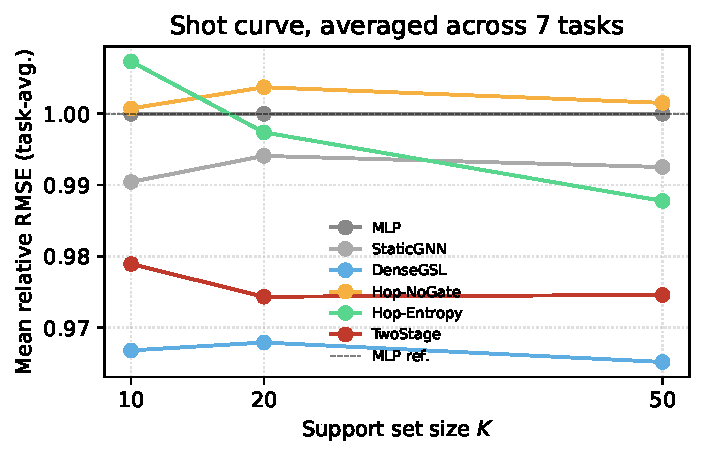
\includegraphics[width=0.96\columnwidth]{figures/shot_curve.pdf}
\caption{Mean relative RMSE (RMSE divided by MLP's RMSE on the same task, then averaged over the seven tasks) as a function of support-set size $K$. Context-augmented conditions improve with $K$; MLP and StaticGNN stay essentially flat at the reference.}
\label{fig:shot_curve}
\end{figure}

\Cref{fig:shot_curve} plots the task-averaged relative RMSE as a function of $K$. The Hopfield-based conditions (Hop-Entropy and TwoStage) separate from the static baselines (MLP, StaticGNN) as $K$ grows, while DenseGSL is already strong at $K=10$ and stays roughly constant. This is consistent with the interpretation that context retrieval's contribution is unlocked more by evidential calibration than by raw retrieval capacity, because the entropy gate becomes sharper once the evidential NIG head has a few support points to anchor on.

\subsection{Per-Task Relative RMSE}

\begin{figure}[t]
\centering
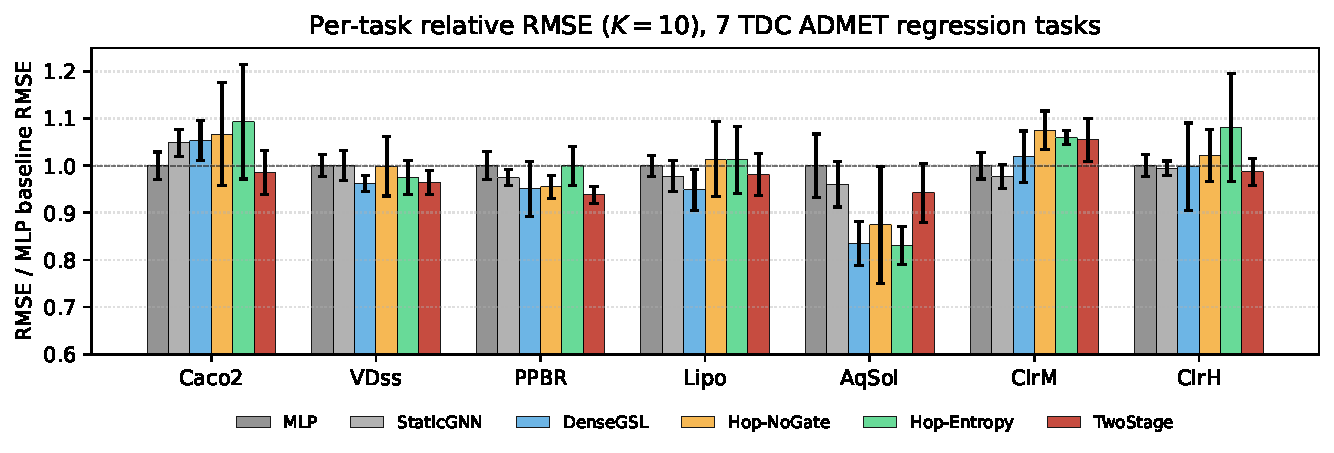
\includegraphics[width=0.99\columnwidth]{figures/per_task_k10.pdf}
\caption{Per-task relative RMSE at $K=10$, normalised by MLP's RMSE on each task. Lower is better. TwoStage (rightmost bar per task group) is below 1.0 on five of seven tasks. Error bars show $\pm 1$ standard deviation across 5 seeds.}
\label{fig:per_task}
\end{figure}

\Cref{fig:per_task} breaks \cref{tab:main_k10} down by task. TwoStage is below the MLP line on five of seven tasks. The two failure cases are both Clearance assays.

\subsection{Failure Analysis: Clearance}

The two Clearance assays behave qualitatively differently from the other five. On Clearance-Microsome, StaticGNN attains the lowest RMSE at both $K$ values, and every context-augmented condition is significantly worse. On Clearance-Hepatocyte, TwoStage recovers the lead at $K\!=\!10$ but Hop-Entropy's per-seed variance (5.68 at $K\!=\!10$) is over three times the TwoStage variance, indicating the entropy gate alone is brittle on this task.

Both Clearance assays have task-level standard deviations (44.8, 49.8) close to the mean MLP RMSE (41.3, 49.4): the typical prediction error is on the order of the data's own spread. In this regime, the gradient signal from any model is dominated by label noise. Retrieval augmentation imports additional noise from the memory bank rather than useful structure. StaticGNN's fixed ECFP graph is the cheapest prior and the one least likely to amplify noise, which is why it wins. TwoStage is therefore not a universal improvement: it is a consistent improvement on ADMET tasks with interpretable structure-activity signal, and loses to simpler baselines on noise-limited assays. This is an honest boundary on the method.

\section{Discussion}
\label{sec:discussion}

\subsection{When Each Gate Helps}

The within-episode evidential gate (DenseGSL) wins cleanly on Lipophilicity and is competitive on VDss and PPBR. Lipophilicity is a local-structure-activity endpoint with a well-populated chemical manifold within any TDC split: the gate's role is simply to suppress the two or three support outliers that a 10-shot sample is likely to contain. Cross-task context adds no signal because the local signal is already dense. This suggests an operational rule: if a task's chemistry is rich and local structure-activity holds, within-episode GSL alone is sufficient.

The combined TwoStage gate wins when cross-task context is informative and support noise is present simultaneously. Caco2 and PPBR are the two clearest cases, and both are tasks where retrieval from the ChEMBL bank actually brings new information: the context molecules are structurally diverse and the endpoints are generalisable enough that ChEMBL neighbours carry task-relevant signal.

\subsection{Why Unconditioned Retrieval Underperforms, and Why Gradient Isolation Matters}

The most robust finding is that Hop-NoGate, our unconditioned-retrieval ablation, never produces the lowest RMSE on any task. Hop-NoGate and Hop-Entropy share the same Hopfield retrieval and learned MolAttention adjacency; only the entropy gate differs. Hop-Entropy's per-seed variance is markedly lower on every task, which indicates the entropy signal is stabilising predictions by ignoring retrievals the model cannot commit to. A cheap zero-parameter gate strictly improves unconditioned retrieval.

An earlier version of our architecture passed the evidential gate through a head fed by the live (not detached) context-enriched features. The support loss's gradient then flowed back into $W_q$, and training became unstable: the retrieval either collapsed (flat $A_{\text{hop}}$) or memorised episode-specific patterns. The stop-gradient on the NIG head's input in \cref{sec:method} is what makes the architecture trainable end-to-end. The broader principle is that cross-task learning and within-task label-noise modelling should share features but not gradients.

\subsection{Relation to MHNfs, ADKF-IFT, and FS-Mol}

We do not run on FS-Mol~\citep{stanley2021fsmol}. FS-Mol is 157 classification tasks reporting $\Delta\text{AUPRC}$; our architecture targets regression, and our NIG head is not the right objective for that benchmark. We see this as complementary rather than a substitute: MHNfs and its successors~\citep{chen2023adkfift,wang2024pintuning,unimatch2025} have defined a standard for classification, while our LOTO-TDC ADMET regression evaluation is, to our knowledge, the first systematic evaluation of the joint retrieval + evidential-gating design on ADMET regression endpoints. A direct apples-to-apples comparison with MHNfs on the same architecture would require porting our FOMAML loop to the FS-Mol support sizes ($K\!\in\!\{16,32,64,128,256\}$) and re-deriving an equivalent classification form of the evidential gate (Dirichlet-based). Both are future work.

We also note a technical distinction from UnGSL~\citep{han2025ungsl}, which combines evidential uncertainty with graph structure learning on transductive node classification. UnGSL places evidential heads on node-level tasks with a fixed graph and no meta-learning, whereas our architecture runs inside a FOMAML loop, adds Hopfield-based cross-task retrieval, and uses gradient isolation to prevent support-loss contamination of the retrieval parameters. The shared mechanism is the evidential-uncertainty gate; the system is otherwise different.

\subsection{Preliminary Classification Results}

Pilot classification runs on two smaller TDC ADMET tasks (HIA-Hou, CYP2C9-Substrate) with a Dirichlet head showed TwoStage (AUROC $0.644{\pm}0.01$ at $K{=}10$; $0.653{\pm}0.01$ at $K{=}50$) statistically indistinguishable from MLP ($0.645{\pm}0.01$; $0.660{\pm}0.01$), while Hop-NoGate was significantly worse ($0.628{\pm}0.01$; $0.635{\pm}0.01$). The Dirichlet aleatoric variance is less informative per sample than the NIG aleatoric mean, so the episode-level gate carries less signal in binary tasks. Reworking stage two for a Dirichlet prior is open.

\subsection{Limitations}

Our evaluation has several acknowledged limitations. Seven regression tasks is moderate; a larger pool would strengthen significance claims. The Clearance-Microsome negative is real and we cannot rule out that task-conditioned retrieval would close it. VDss-Lombardo shows elevated seed-level variance at $K{\in}\{20,50\}$ because seed 2 converges to a markedly lower RMSE ($\sim14$) than seeds $\{0,1,3,4\}$ ($\sim24$--$28$) across every condition; the paired-$t$ test is robust to the shift but absolute means are pulled by that seed. We did not run a context-set-size ablation. Finally, Hop-NoGate is not a real MHNfs reference run, as explained in \cref{sec:experiments}.

On compute: a full LOTO run over 7 folds, 6 conditions, 5 seeds takes $\sim$38 GPU-hours on a single A100, dominated by meta-training. Meta-test is negligible. The ChEMBL 50k context occupies $\sim$150 MB of GPU memory once projected.

\section{Conclusion}
\label{sec:conclusion}

We presented a few-shot meta-learning architecture that combines Modern Hopfield retrieval with evidential graph structure learning through a two-stage uncertainty gate: a zero-parameter entropy gate that suppresses diffuse retrievals, and a gradient-isolated evidential gate that suppresses poorly-fit supports. Both gates are necessary; their combination is the only condition that wins on multiple TDC ADMET regression tasks at both $K\!=\!10$ and $K\!=\!50$, while unconditioned Hopfield retrieval never wins. The Clearance-Microsome negative is a boundary condition: on noise-limited assays, retrieval augmentation cannot help. The operational rule is a mixture: within-episode evidential GSL for tasks with dense local chemistry, the two-stage gate when cross-task context is informative, and simpler baselines on assays whose label variance approaches the target scale.

\bibliography{paper}
\bibliographystyle{icml2026}

\end{document}
